% Options for packages loaded elsewhere
\PassOptionsToPackage{unicode}{hyperref}
\PassOptionsToPackage{hyphens}{url}
%
\documentclass[
]{article}
\usepackage{lmodern}
\usepackage{amssymb,amsmath}
\usepackage{ifxetex,ifluatex}
\ifnum 0\ifxetex 1\fi\ifluatex 1\fi=0 % if pdftex
  \usepackage[T1]{fontenc}
  \usepackage[utf8]{inputenc}
  \usepackage{textcomp} % provide euro and other symbols
\else % if luatex or xetex
  \usepackage{unicode-math}
  \defaultfontfeatures{Scale=MatchLowercase}
  \defaultfontfeatures[\rmfamily]{Ligatures=TeX,Scale=1}
\fi
% Use upquote if available, for straight quotes in verbatim environments
\IfFileExists{upquote.sty}{\usepackage{upquote}}{}
\IfFileExists{microtype.sty}{% use microtype if available
  \usepackage[]{microtype}
  \UseMicrotypeSet[protrusion]{basicmath} % disable protrusion for tt fonts
}{}
\makeatletter
\@ifundefined{KOMAClassName}{% if non-KOMA class
  \IfFileExists{parskip.sty}{%
    \usepackage{parskip}
  }{% else
    \setlength{\parindent}{0pt}
    \setlength{\parskip}{6pt plus 2pt minus 1pt}}
}{% if KOMA class
  \KOMAoptions{parskip=half}}
\makeatother
\usepackage{xcolor}
\IfFileExists{xurl.sty}{\usepackage{xurl}}{} % add URL line breaks if available
\IfFileExists{bookmark.sty}{\usepackage{bookmark}}{\usepackage{hyperref}}
\hypersetup{
  pdftitle={Compulsory exercise 3},
  pdfauthor={Sara Elise Wøllo)},
  hidelinks,
  pdfcreator={LaTeX via pandoc}}
\urlstyle{same} % disable monospaced font for URLs
\usepackage[margin=1in]{geometry}
\usepackage{color}
\usepackage{fancyvrb}
\newcommand{\VerbBar}{|}
\newcommand{\VERB}{\Verb[commandchars=\\\{\}]}
\DefineVerbatimEnvironment{Highlighting}{Verbatim}{commandchars=\\\{\}}
% Add ',fontsize=\small' for more characters per line
\usepackage{framed}
\definecolor{shadecolor}{RGB}{248,248,248}
\newenvironment{Shaded}{\begin{snugshade}}{\end{snugshade}}
\newcommand{\AlertTok}[1]{\textcolor[rgb]{0.94,0.16,0.16}{#1}}
\newcommand{\AnnotationTok}[1]{\textcolor[rgb]{0.56,0.35,0.01}{\textbf{\textit{#1}}}}
\newcommand{\AttributeTok}[1]{\textcolor[rgb]{0.77,0.63,0.00}{#1}}
\newcommand{\BaseNTok}[1]{\textcolor[rgb]{0.00,0.00,0.81}{#1}}
\newcommand{\BuiltInTok}[1]{#1}
\newcommand{\CharTok}[1]{\textcolor[rgb]{0.31,0.60,0.02}{#1}}
\newcommand{\CommentTok}[1]{\textcolor[rgb]{0.56,0.35,0.01}{\textit{#1}}}
\newcommand{\CommentVarTok}[1]{\textcolor[rgb]{0.56,0.35,0.01}{\textbf{\textit{#1}}}}
\newcommand{\ConstantTok}[1]{\textcolor[rgb]{0.00,0.00,0.00}{#1}}
\newcommand{\ControlFlowTok}[1]{\textcolor[rgb]{0.13,0.29,0.53}{\textbf{#1}}}
\newcommand{\DataTypeTok}[1]{\textcolor[rgb]{0.13,0.29,0.53}{#1}}
\newcommand{\DecValTok}[1]{\textcolor[rgb]{0.00,0.00,0.81}{#1}}
\newcommand{\DocumentationTok}[1]{\textcolor[rgb]{0.56,0.35,0.01}{\textbf{\textit{#1}}}}
\newcommand{\ErrorTok}[1]{\textcolor[rgb]{0.64,0.00,0.00}{\textbf{#1}}}
\newcommand{\ExtensionTok}[1]{#1}
\newcommand{\FloatTok}[1]{\textcolor[rgb]{0.00,0.00,0.81}{#1}}
\newcommand{\FunctionTok}[1]{\textcolor[rgb]{0.00,0.00,0.00}{#1}}
\newcommand{\ImportTok}[1]{#1}
\newcommand{\InformationTok}[1]{\textcolor[rgb]{0.56,0.35,0.01}{\textbf{\textit{#1}}}}
\newcommand{\KeywordTok}[1]{\textcolor[rgb]{0.13,0.29,0.53}{\textbf{#1}}}
\newcommand{\NormalTok}[1]{#1}
\newcommand{\OperatorTok}[1]{\textcolor[rgb]{0.81,0.36,0.00}{\textbf{#1}}}
\newcommand{\OtherTok}[1]{\textcolor[rgb]{0.56,0.35,0.01}{#1}}
\newcommand{\PreprocessorTok}[1]{\textcolor[rgb]{0.56,0.35,0.01}{\textit{#1}}}
\newcommand{\RegionMarkerTok}[1]{#1}
\newcommand{\SpecialCharTok}[1]{\textcolor[rgb]{0.00,0.00,0.00}{#1}}
\newcommand{\SpecialStringTok}[1]{\textcolor[rgb]{0.31,0.60,0.02}{#1}}
\newcommand{\StringTok}[1]{\textcolor[rgb]{0.31,0.60,0.02}{#1}}
\newcommand{\VariableTok}[1]{\textcolor[rgb]{0.00,0.00,0.00}{#1}}
\newcommand{\VerbatimStringTok}[1]{\textcolor[rgb]{0.31,0.60,0.02}{#1}}
\newcommand{\WarningTok}[1]{\textcolor[rgb]{0.56,0.35,0.01}{\textbf{\textit{#1}}}}
\usepackage{graphicx,grffile}
\makeatletter
\def\maxwidth{\ifdim\Gin@nat@width>\linewidth\linewidth\else\Gin@nat@width\fi}
\def\maxheight{\ifdim\Gin@nat@height>\textheight\textheight\else\Gin@nat@height\fi}
\makeatother
% Scale images if necessary, so that they will not overflow the page
% margins by default, and it is still possible to overwrite the defaults
% using explicit options in \includegraphics[width, height, ...]{}
\setkeys{Gin}{width=\maxwidth,height=\maxheight,keepaspectratio}
% Set default figure placement to htbp
\makeatletter
\def\fps@figure{htbp}
\makeatother
\setlength{\emergencystretch}{3em} % prevent overfull lines
\providecommand{\tightlist}{%
  \setlength{\itemsep}{0pt}\setlength{\parskip}{0pt}}
\setcounter{secnumdepth}{-\maxdimen} % remove section numbering

\title{Compulsory exercise 3}
\usepackage{etoolbox}
\makeatletter
\providecommand{\subtitle}[1]{% add subtitle to \maketitle
  \apptocmd{\@title}{\par {\large #1 \par}}{}{}
}
\makeatother
\subtitle{TMA4268 Statistical Learning V2019}
\author{Sara Elise Wøllo)}
\date{19 4 2020}

\begin{document}
\maketitle

\hypertarget{problem-1}{%
\section{Problem 1}\label{problem-1}}

\hypertarget{a}{%
\subsection{a)}\label{a}}

\begin{Shaded}
\begin{Highlighting}[]
\KeywordTok{set.seed}\NormalTok{(}\DecValTok{1}\NormalTok{)}
\NormalTok{College}\OperatorTok{$}\NormalTok{Private =}\StringTok{ }\KeywordTok{as.numeric}\NormalTok{(College}\OperatorTok{$}\NormalTok{Private)}
\NormalTok{train.ind =}\StringTok{ }\KeywordTok{sample}\NormalTok{(}\DecValTok{1}\OperatorTok{:}\KeywordTok{nrow}\NormalTok{(College), }\FloatTok{0.5} \OperatorTok{*}\StringTok{ }\KeywordTok{nrow}\NormalTok{(College))}
\NormalTok{college.train =}\StringTok{ }\NormalTok{College[train.ind, ]}
\NormalTok{college.test =}\StringTok{ }\NormalTok{College[}\OperatorTok{-}\NormalTok{train.ind, ]}
\KeywordTok{str}\NormalTok{(college.train)}
\end{Highlighting}
\end{Shaded}

\begin{verbatim}
## 'data.frame':    388 obs. of  18 variables:
##  $ Private    : num  1 2 1 2 2 1 2 2 2 2 ...
##  $ Apps       : num  1401 344 4216 427 2929 ...
##  $ Accept     : num  1239 264 2290 385 1834 ...
##  $ Enroll     : num  605 97 736 143 622 ...
##  $ Top10perc  : num  10 11 20 18 20 10 27 50 62 13 ...
##  $ Top25perc  : num  34 42 52 38 56 35 50 77 93 33 ...
##  $ F.Undergrad: num  3716 500 4296 581 2738 ...
##  $ P.Undergrad: num  675 331 1027 533 1662 ...
##  $ Outstate   : num  7100 12600 5130 12700 12600 ...
##  $ Room.Board : num  4380 5520 4690 5800 5610 ...
##  $ Books      : num  540 630 600 450 450 537 450 525 500 570 ...
##  $ Personal   : num  2948 2250 1450 700 3160 ...
##  $ PhD        : num  63 77 73 81 90 77 77 76 94 66 ...
##  $ Terminal   : num  88 80 75 85 90 84 98 92 96 83 ...
##  $ S.F.Ratio  : num  19.4 10.4 17.9 10.3 15.1 21 21.5 10.1 9.6 16 ...
##  $ perc.alumni: num  0 7 18 37 9 16 21 57 20 14 ...
##  $ Expend     : num  5389 9773 5125 11758 9084 ...
##  $ Grad.Rate  : num  36 43 56 84 84 54 64 77 93 66 ...
\end{verbatim}

\begin{Shaded}
\begin{Highlighting}[]
\NormalTok{outstate.train =}\StringTok{ }\KeywordTok{subset}\NormalTok{(college.train, }\DataTypeTok{select =} \KeywordTok{c}\NormalTok{(Outstate))}
\NormalTok{outstate.test =}\StringTok{ }\KeywordTok{subset}\NormalTok{(college.test, }\DataTypeTok{select =} \KeywordTok{c}\NormalTok{(Outstate))}
\NormalTok{college.train =}\StringTok{ }\KeywordTok{subset}\NormalTok{(college.train, }\DataTypeTok{select =} \OperatorTok{-}\KeywordTok{c}\NormalTok{(Outstate))}
\NormalTok{college.test =}\StringTok{ }\KeywordTok{subset}\NormalTok{(college.test, }\DataTypeTok{select =} \OperatorTok{-}\KeywordTok{c}\NormalTok{(Outstate))}

\NormalTok{mean <-}\StringTok{ }\KeywordTok{apply}\NormalTok{(college.train, }\DecValTok{2}\NormalTok{, mean)}
\NormalTok{std <-}\StringTok{ }\KeywordTok{apply}\NormalTok{(college.train, }\DecValTok{2}\NormalTok{, sd)}
\NormalTok{college.train <-}\StringTok{ }\KeywordTok{scale}\NormalTok{(college.train, }\DataTypeTok{center =}\NormalTok{ mean, }\DataTypeTok{scale =}\NormalTok{ std)}
\NormalTok{college.test <-}\StringTok{ }\KeywordTok{scale}\NormalTok{(college.test, }\DataTypeTok{center =}\NormalTok{ mean, }\DataTypeTok{scale =}\NormalTok{ std)}
\end{Highlighting}
\end{Shaded}

\hypertarget{b}{%
\subsection{b)}\label{b}}

\$\$

y\_1 =\Big(1 + \exp \Big( -\beta\emph{\{01\} - \sum}\{m=1\}\^{}\{64\}
\beta\emph{\{m1\} max \Big( \gamma}\{0m\}\sum\emph{\{l=1\}\^{}\{64\}
\gamma}\{lm\} max \Big(
\alpha\emph{\{0l\}\sum}\{j=1\}\^{}\{17\}\alpha\_\{jl\}x\_j,0
\Big),0\Big) \Big)\^{}\{-1\}\Big) \$\$ Using Sigmoid activation on the
output layer. \#\# c)

\begin{Shaded}
\begin{Highlighting}[]
\CommentTok{# set.seed(1) train.in = sample(1:nrow(college.train), 0.8 * nrow(college.train))}
\CommentTok{# college.train1 = college.train[train.in, ] college.vali =}
\CommentTok{# college.train[-train.in, ] str(college.train1)}
\end{Highlighting}
\end{Shaded}

\begin{Shaded}
\begin{Highlighting}[]
\NormalTok{model =}\StringTok{ }\KeywordTok{keras_model_sequential}\NormalTok{() }\OperatorTok\StringTok{ }\KeywordTok{layer_dense}\NormalTok{(}\DataTypeTok{units =} \DecValTok{64}\NormalTok{, }\DataTypeTok{activation =} \StringTok{"relu"}\NormalTok{, }
    \DataTypeTok{input_shape =} \KeywordTok{c}\NormalTok{(}\DecValTok{388}\NormalTok{)) }\OperatorTok\StringTok{ }\KeywordTok{layer_dense}\NormalTok{(}\DataTypeTok{units =} \DecValTok{64}\NormalTok{, }\DataTypeTok{activation =} \StringTok{"relu"}\NormalTok{) }\OperatorTok\StringTok{ }\KeywordTok{layer_dense}\NormalTok{(}\DataTypeTok{units =} \DecValTok{1}\NormalTok{, }
    \DataTypeTok{activation =} \StringTok{"sigmoid"}\NormalTok{)}
\end{Highlighting}
\end{Shaded}

\begin{Shaded}
\begin{Highlighting}[]
\NormalTok{model }\OperatorTok\StringTok{ }\KeywordTok{compile}\NormalTok{(}\DataTypeTok{optimizer =} \StringTok{"rmsprop"}\NormalTok{, }\DataTypeTok{loss =} \StringTok{"binary_crossentropy"}\NormalTok{, }\DataTypeTok{metrics =} \KeywordTok{c}\NormalTok{(}\StringTok{"accuracy"}\NormalTok{))}
\end{Highlighting}
\end{Shaded}

\begin{Shaded}
\begin{Highlighting}[]
\CommentTok{# set.seed(123) history = model %>% fit(college.train$x,college.train$y, epochs =}
\CommentTok{# 300, batch_size = 8, validation_split = 0.2) str(history)}
\end{Highlighting}
\end{Shaded}

\hypertarget{d}{%
\subsection{d)}\label{d}}

\hypertarget{problem-2}{%
\section{Problem 2}\label{problem-2}}

\begin{Shaded}
\begin{Highlighting}[]
\NormalTok{id <-}\StringTok{ "1CA1RPRYqU9oTIaHfSroitnWrI6WpUeBw"}  \CommentTok{# google file ID}
\NormalTok{d.corona <-}\StringTok{ }\KeywordTok{read.csv}\NormalTok{(}\KeywordTok{sprintf}\NormalTok{(}\StringTok{"https://docs.google.com/uc?id=%s&export=download"}\NormalTok{, }
\NormalTok{    id), }\DataTypeTok{header =}\NormalTok{ T)}
\end{Highlighting}
\end{Shaded}

\hypertarget{a-1}{%
\subsection{a)}\label{a-1}}

\begin{Shaded}
\begin{Highlighting}[]
\KeywordTok{count}\NormalTok{(d.corona, country, deceased)}
\end{Highlighting}
\end{Shaded}

\begin{verbatim}
## # A tibble: 8 x 3
##   country   deceased     n
##   <fct>        <int> <int>
## 1 France           0   100
## 2 France           1    14
## 3 indonesia        0    67
## 4 indonesia        1     2
## 5 japan            0   291
## 6 japan            1     3
## 7 Korea            0  1507
## 8 Korea            1    26
\end{verbatim}

\begin{Shaded}
\begin{Highlighting}[]
\KeywordTok{count}\NormalTok{(d.corona, sex, deceased)}
\end{Highlighting}
\end{Shaded}

\begin{verbatim}
## # A tibble: 4 x 3
##   sex    deceased     n
##   <fct>     <int> <int>
## 1 female        0  1075
## 2 female        1    14
## 3 male          0   890
## 4 male          1    31
\end{verbatim}

\begin{Shaded}
\begin{Highlighting}[]
\KeywordTok{count}\NormalTok{(d.corona, country, sex, deceased)}
\end{Highlighting}
\end{Shaded}

\begin{verbatim}
## # A tibble: 15 x 4
##    country   sex    deceased     n
##    <fct>     <fct>     <int> <int>
##  1 France    female        0    55
##  2 France    female        1     5
##  3 France    male          0    45
##  4 France    male          1     9
##  5 indonesia female        0    29
##  6 indonesia female        1     1
##  7 indonesia male          0    38
##  8 indonesia male          1     1
##  9 japan     female        0   120
## 10 japan     male          0   171
## 11 japan     male          1     3
## 12 Korea     female        0   871
## 13 Korea     female        1     8
## 14 Korea     male          0   636
## 15 Korea     male          1    18
\end{verbatim}

We see that there are 14 (5 female (f), 9 male (m)) deceased in France,
2 (1 (f), 1 (m)) in Indonesia, 3 (0 (f), 3 (m)) in Japan and 26 ( 8(f),
18 (m)) in Korea. There are 14 females deceased and 31 males deceased.

\hypertarget{b-1}{%
\subsection{b)}\label{b-1}}

Kan (kanskje) løse den brute force, men det er lite elegant.

\begin{Shaded}
\begin{Highlighting}[]
\NormalTok{fit <-}\StringTok{ }\KeywordTok{glm}\NormalTok{(deceased }\OperatorTok{~}\StringTok{ }\NormalTok{sex }\OperatorTok{+}\StringTok{ }\NormalTok{age }\OperatorTok{+}\StringTok{ }\NormalTok{country, }\DataTypeTok{data =}\NormalTok{ d.corona, }\DataTypeTok{family =} \StringTok{"binomial"}\NormalTok{)}
\NormalTok{fit}
\end{Highlighting}
\end{Shaded}

\begin{verbatim}
## 
## Call:  glm(formula = deceased ~ sex + age + country, family = "binomial", 
##     data = d.corona)
## 
## Coefficients:
##      (Intercept)           sexmale               age  countryindonesia  
##         -7.63305           1.13725           0.06801          -0.75426  
##     countryjapan      countryKorea  
##         -2.43410          -1.36680  
## 
## Degrees of Freedom: 2009 Total (i.e. Null);  2004 Residual
## Null Deviance:       430.9 
## Residual Deviance: 321.1     AIC: 333.1
\end{verbatim}

\begin{Shaded}
\begin{Highlighting}[]
\KeywordTok{ggplot}\NormalTok{(}\DataTypeTok{data =}\NormalTok{ d.corona, }\KeywordTok{aes}\NormalTok{(age, deceased)) }\OperatorTok{+}\StringTok{ }\KeywordTok{geom_point}\NormalTok{()}
\end{Highlighting}
\end{Shaded}

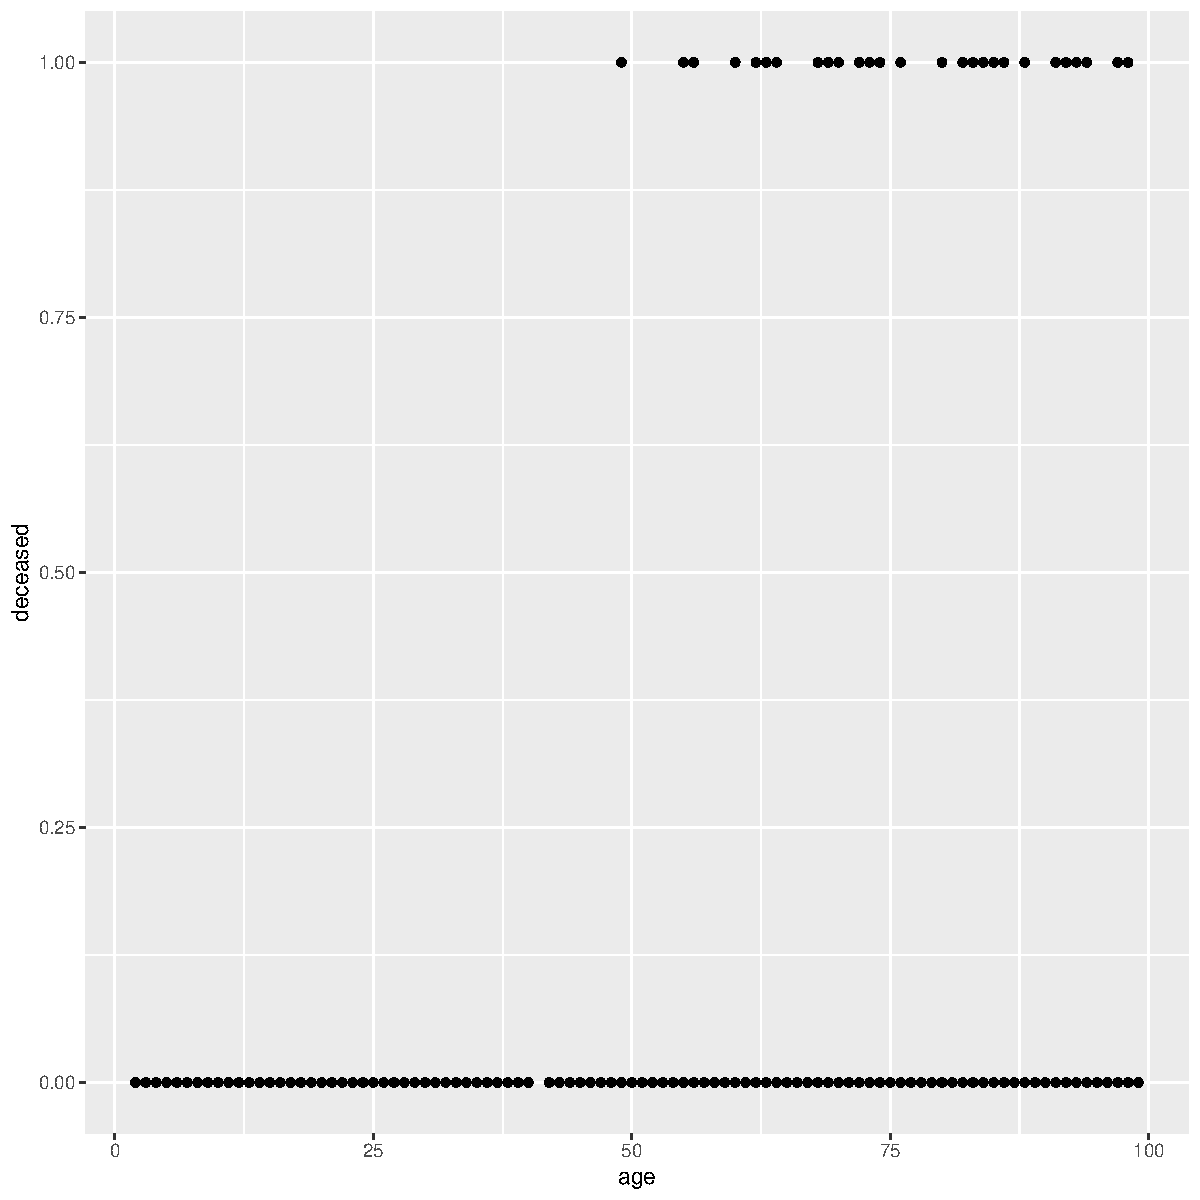
\includegraphics{Eksamensbesvarelse_files/figure-latex/unnamed-chunk-8-1.pdf}

\begin{Shaded}
\begin{Highlighting}[]
\KeywordTok{summary}\NormalTok{(fit)}
\end{Highlighting}
\end{Shaded}

\begin{verbatim}
## 
## Call:
## glm(formula = deceased ~ sex + age + country, family = "binomial", 
##     data = d.corona)
## 
## Deviance Residuals: 
##     Min       1Q   Median       3Q      Max  
## -1.2797  -0.1855  -0.1009  -0.0553   3.2233  
## 
## Coefficients:
##                   Estimate Std. Error z value Pr(>|z|)    
## (Intercept)      -7.633051   0.897063  -8.509  < 2e-16 ***
## sexmale           1.137246   0.343706   3.309 0.000937 ***
## age               0.068012   0.009846   6.907 4.94e-12 ***
## countryindonesia -0.754259   0.815127  -0.925 0.354796    
## countryjapan     -2.434101   0.667826  -3.645 0.000268 ***
## countryKorea     -1.366797   0.374837  -3.646 0.000266 ***
## ---
## Signif. codes:  0 '***' 0.001 '**' 0.01 '*' 0.05 '.' 0.1 ' ' 1
## 
## (Dispersion parameter for binomial family taken to be 1)
## 
##     Null deviance: 430.92  on 2009  degrees of freedom
## Residual deviance: 321.07  on 2004  degrees of freedom
## AIC: 333.07
## 
## Number of Fisher Scoring iterations: 8
\end{verbatim}

\begin{enumerate}
\def\labelenumi{\roman{enumi})}
\tightlist
\item
  False? It is split into several covaraiates in the model ii) False?
  Don't need to remove from model even though it is not sig. iii) True
  iv) True
\end{enumerate}

:::iii) Odds ratio

\begin{Shaded}
\begin{Highlighting}[]
\NormalTok{eta =}\StringTok{ }\FloatTok{-7.633051} \OperatorTok{+}\StringTok{ }\NormalTok{(}\FloatTok{1.137246} \OperatorTok{*}\StringTok{ }\DecValTok{1}\NormalTok{) }\OperatorTok{+}\StringTok{ }\NormalTok{(}\FloatTok{0.068012} \OperatorTok{*}\StringTok{ }\DecValTok{31}\NormalTok{) }\OperatorTok{-}\StringTok{ }\NormalTok{(}\FloatTok{0.754259} \OperatorTok{*}\StringTok{ }\DecValTok{0}\NormalTok{) }\OperatorTok{-}\StringTok{ }\NormalTok{(}\FloatTok{2.434101} \OperatorTok{*}\StringTok{ }
\StringTok{    }\DecValTok{1}\NormalTok{) }\OperatorTok{-}\StringTok{ }\NormalTok{(}\FloatTok{1.366797} \OperatorTok{*}\StringTok{ }\DecValTok{0}\NormalTok{)}


\NormalTok{newdata =}\StringTok{ }\KeywordTok{exp}\NormalTok{(eta)}\OperatorTok{/}\NormalTok{(}\DecValTok{1} \OperatorTok{+}\StringTok{ }\KeywordTok{exp}\NormalTok{(eta))}
\NormalTok{newdata}
\end{Highlighting}
\end{Shaded}

\begin{verbatim}
## [1] 0.001088861
\end{verbatim}

\begin{Shaded}
\begin{Highlighting}[]
\NormalTok{odds =}\StringTok{ }\NormalTok{newdata}\OperatorTok{/}\NormalTok{(}\DecValTok{1} \OperatorTok{-}\StringTok{ }\NormalTok{newdata)}
\NormalTok{odds}
\end{Highlighting}
\end{Shaded}

\begin{verbatim}
## [1] 0.001090048
\end{verbatim}

\hypertarget{c}{%
\subsection{c)}\label{c}}

\begin{Shaded}
\begin{Highlighting}[]
\NormalTok{grid_fr_m =}\StringTok{ }\KeywordTok{expand.grid}\NormalTok{(}\DataTypeTok{sex =} \StringTok{"male"}\NormalTok{, }\DataTypeTok{age =} \KeywordTok{seq}\NormalTok{(}\DecValTok{20}\NormalTok{, }\DecValTok{100}\NormalTok{, }\DecValTok{1}\NormalTok{), }\DataTypeTok{country =} \StringTok{"France"}\NormalTok{)}
\NormalTok{grid_fr_f =}\StringTok{ }\KeywordTok{expand.grid}\NormalTok{(}\DataTypeTok{sex =} \StringTok{"female"}\NormalTok{, }\DataTypeTok{age =} \KeywordTok{seq}\NormalTok{(}\DecValTok{20}\NormalTok{, }\DecValTok{100}\NormalTok{, }\DecValTok{1}\NormalTok{), }\DataTypeTok{country =} \StringTok{"France"}\NormalTok{)}
\NormalTok{grid_in_m =}\StringTok{ }\KeywordTok{expand.grid}\NormalTok{(}\DataTypeTok{sex =} \StringTok{"male"}\NormalTok{, }\DataTypeTok{age =} \KeywordTok{seq}\NormalTok{(}\DecValTok{20}\NormalTok{, }\DecValTok{100}\NormalTok{, }\DecValTok{1}\NormalTok{), }\DataTypeTok{country =} \StringTok{"indonesia"}\NormalTok{)}
\NormalTok{grid_in_f =}\StringTok{ }\KeywordTok{expand.grid}\NormalTok{(}\DataTypeTok{sex =} \StringTok{"female"}\NormalTok{, }\DataTypeTok{age =} \KeywordTok{seq}\NormalTok{(}\DecValTok{20}\NormalTok{, }\DecValTok{100}\NormalTok{, }\DecValTok{1}\NormalTok{), }\DataTypeTok{country =} \StringTok{"indonesia"}\NormalTok{)}
\NormalTok{grid_ja_m =}\StringTok{ }\KeywordTok{expand.grid}\NormalTok{(}\DataTypeTok{sex =} \StringTok{"male"}\NormalTok{, }\DataTypeTok{age =} \KeywordTok{seq}\NormalTok{(}\DecValTok{20}\NormalTok{, }\DecValTok{100}\NormalTok{, }\DecValTok{1}\NormalTok{), }\DataTypeTok{country =} \StringTok{"japan"}\NormalTok{)}
\NormalTok{grid_ja_f =}\StringTok{ }\KeywordTok{expand.grid}\NormalTok{(}\DataTypeTok{sex =} \StringTok{"female"}\NormalTok{, }\DataTypeTok{age =} \KeywordTok{seq}\NormalTok{(}\DecValTok{20}\NormalTok{, }\DecValTok{100}\NormalTok{, }\DecValTok{1}\NormalTok{), }\DataTypeTok{country =} \StringTok{"japan"}\NormalTok{)}
\NormalTok{grid_ko_m =}\StringTok{ }\KeywordTok{expand.grid}\NormalTok{(}\DataTypeTok{sex =} \StringTok{"male"}\NormalTok{, }\DataTypeTok{age =} \KeywordTok{seq}\NormalTok{(}\DecValTok{20}\NormalTok{, }\DecValTok{100}\NormalTok{, }\DecValTok{1}\NormalTok{), }\DataTypeTok{country =} \StringTok{"Korea"}\NormalTok{)}
\NormalTok{grid_ko_f =}\StringTok{ }\KeywordTok{expand.grid}\NormalTok{(}\DataTypeTok{sex =} \StringTok{"female"}\NormalTok{, }\DataTypeTok{age =} \KeywordTok{seq}\NormalTok{(}\DecValTok{20}\NormalTok{, }\DecValTok{100}\NormalTok{, }\DecValTok{1}\NormalTok{), }\DataTypeTok{country =} \StringTok{"Korea"}\NormalTok{)}

\NormalTok{m_france =}\StringTok{ }\KeywordTok{predict.glm}\NormalTok{(fit, }\DataTypeTok{newdata =}\NormalTok{ grid_fr_m, }\DataTypeTok{type =} \StringTok{"response"}\NormalTok{)}
\NormalTok{f_france =}\StringTok{ }\KeywordTok{predict.glm}\NormalTok{(fit, }\DataTypeTok{newdata =}\NormalTok{ grid_fr_f, }\DataTypeTok{type =} \StringTok{"response"}\NormalTok{)}
\NormalTok{m_indo =}\StringTok{ }\KeywordTok{predict.glm}\NormalTok{(fit, }\DataTypeTok{newdata =}\NormalTok{ grid_in_m, }\DataTypeTok{type =} \StringTok{"response"}\NormalTok{)}
\NormalTok{f_indo =}\StringTok{ }\KeywordTok{predict.glm}\NormalTok{(fit, }\DataTypeTok{newdata =}\NormalTok{ grid_in_f, }\DataTypeTok{type =} \StringTok{"response"}\NormalTok{)}
\NormalTok{m_japan =}\StringTok{ }\KeywordTok{predict.glm}\NormalTok{(fit, }\DataTypeTok{newdata =}\NormalTok{ grid_ja_m, }\DataTypeTok{type =} \StringTok{"response"}\NormalTok{)}
\NormalTok{f_japan =}\StringTok{ }\KeywordTok{predict.glm}\NormalTok{(fit, }\DataTypeTok{newdata =}\NormalTok{ grid_ja_f, }\DataTypeTok{type =} \StringTok{"response"}\NormalTok{)}
\NormalTok{m_korea =}\StringTok{ }\KeywordTok{predict.glm}\NormalTok{(fit, }\DataTypeTok{newdata =}\NormalTok{ grid_ko_m, }\DataTypeTok{type =} \StringTok{"response"}\NormalTok{)}
\NormalTok{f_korea =}\StringTok{ }\KeywordTok{predict.glm}\NormalTok{(fit, }\DataTypeTok{newdata =}\NormalTok{ grid_ko_f, }\DataTypeTok{type =} \StringTok{"response"}\NormalTok{)}
\end{Highlighting}
\end{Shaded}

\begin{Shaded}
\begin{Highlighting}[]
\KeywordTok{plot}\NormalTok{(m_france, }\DataTypeTok{type =} \StringTok{"l"}\NormalTok{, }\DataTypeTok{lwd =} \DecValTok{1}\NormalTok{, }\DataTypeTok{col =} \DecValTok{1}\NormalTok{, }\DataTypeTok{xlab =} \StringTok{"Age"}\NormalTok{, }\DataTypeTok{ylab =} \StringTok{"Probability of death"}\NormalTok{)}
\KeywordTok{lines}\NormalTok{(f_france, }\DataTypeTok{lwd =} \DecValTok{1}\NormalTok{, }\DataTypeTok{col =} \DecValTok{2}\NormalTok{)}
\KeywordTok{lines}\NormalTok{(m_indo, }\DataTypeTok{lwd =} \DecValTok{1}\NormalTok{, }\DataTypeTok{col =} \DecValTok{3}\NormalTok{)}
\KeywordTok{lines}\NormalTok{(f_indo, }\DataTypeTok{lwd =} \DecValTok{1}\NormalTok{, }\DataTypeTok{col =} \DecValTok{4}\NormalTok{)}
\KeywordTok{lines}\NormalTok{(m_japan, }\DataTypeTok{lwd =} \DecValTok{1}\NormalTok{, }\DataTypeTok{col =} \DecValTok{5}\NormalTok{)}
\KeywordTok{lines}\NormalTok{(f_japan, }\DataTypeTok{lwd =} \DecValTok{1}\NormalTok{, }\DataTypeTok{col =} \DecValTok{6}\NormalTok{)}
\KeywordTok{lines}\NormalTok{(m_korea, }\DataTypeTok{lwd =} \DecValTok{1}\NormalTok{, }\DataTypeTok{col =} \DecValTok{7}\NormalTok{)}
\KeywordTok{lines}\NormalTok{(f_korea, }\DataTypeTok{lwd =} \DecValTok{1}\NormalTok{, }\DataTypeTok{col =} \DecValTok{8}\NormalTok{)}
\KeywordTok{title}\NormalTok{(}\StringTok{"Probability to die of Coronavirus, for country and sex"}\NormalTok{)}
\KeywordTok{legend}\NormalTok{(}\DataTypeTok{x =} \StringTok{"topleft"}\NormalTok{, }\DataTypeTok{legend =} \KeywordTok{c}\NormalTok{(}\StringTok{"France,m"}\NormalTok{, }\StringTok{"France,f"}\NormalTok{, }\StringTok{"Indonesia,m"}\NormalTok{, }\StringTok{"Indonesia,f"}\NormalTok{, }
    \StringTok{"Japan,m"}\NormalTok{, }\StringTok{"Japan,f"}\NormalTok{, }\StringTok{"Korea,m"}\NormalTok{, }\StringTok{"Korea,f"}\NormalTok{), }\DataTypeTok{lwd =} \KeywordTok{c}\NormalTok{(}\DecValTok{2}\NormalTok{, }\DecValTok{2}\NormalTok{, }\DecValTok{2}\NormalTok{, }\DecValTok{2}\NormalTok{, }\DecValTok{2}\NormalTok{, }\DecValTok{2}\NormalTok{, }\DecValTok{2}\NormalTok{, }\DecValTok{2}\NormalTok{), }
    \DataTypeTok{col =} \KeywordTok{c}\NormalTok{(}\DecValTok{1}\NormalTok{, }\DecValTok{2}\NormalTok{, }\DecValTok{3}\NormalTok{, }\DecValTok{4}\NormalTok{, }\DecValTok{5}\NormalTok{, }\DecValTok{6}\NormalTok{, }\DecValTok{7}\NormalTok{, }\DecValTok{8}\NormalTok{), }\DataTypeTok{y.intersp =} \DecValTok{1}\NormalTok{)}
\end{Highlighting}
\end{Shaded}

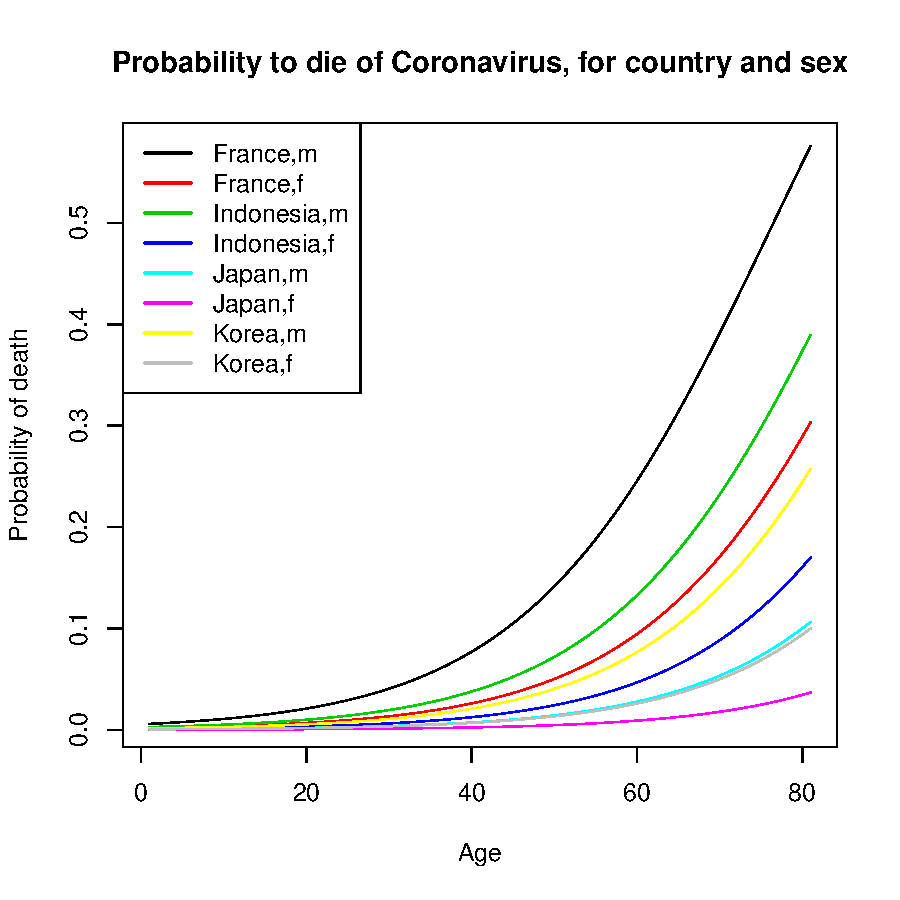
\includegraphics{Eksamensbesvarelse_files/figure-latex/unnamed-chunk-11-1.pdf}

\hypertarget{d-should-i-fit-one-more-model}{%
\subsection{d) {[}should I fit one more
model?{]}}\label{d-should-i-fit-one-more-model}}

\begin{enumerate}
\def\labelenumi{\roman{enumi})}
\tightlist
\item
  True. As you see from the plot ``Probability to die of Coronavirus,
  for sex''. Add \ref{}. Males have higher probability of death.
\item
  Yes? At a low age, the mortality rates are similar, but at age
  increases, the mortality rates increases faster for men than for
  women.
\item
  Yes? The mortality rate for the Frence population is higher even at
  low ages, but the difference increases as age increaces.
\end{enumerate}

\begin{Shaded}
\begin{Highlighting}[]
\NormalTok{fit <-}\StringTok{ }\KeywordTok{glm}\NormalTok{(deceased }\OperatorTok{~}\StringTok{ }\NormalTok{sex }\OperatorTok{+}\StringTok{ }\NormalTok{age, }\DataTypeTok{data =}\NormalTok{ d.corona, }\DataTypeTok{family =} \StringTok{"binomial"}\NormalTok{)}
\NormalTok{fit}
\end{Highlighting}
\end{Shaded}

\begin{verbatim}
## 
## Call:  glm(formula = deceased ~ sex + age, family = "binomial", data = d.corona)
## 
## Coefficients:
## (Intercept)      sexmale          age  
##    -9.06638      1.06696      0.07119  
## 
## Degrees of Freedom: 2009 Total (i.e. Null);  2007 Residual
## Null Deviance:       430.9 
## Residual Deviance: 340.4     AIC: 346.4
\end{verbatim}

\begin{Shaded}
\begin{Highlighting}[]
\NormalTok{fit_country <-}\StringTok{ }\KeywordTok{glm}\NormalTok{(deceased }\OperatorTok{~}\StringTok{ }\NormalTok{age }\OperatorTok{+}\StringTok{ }\NormalTok{country, }\DataTypeTok{data =}\NormalTok{ d.corona, }\DataTypeTok{family =} \StringTok{"binomial"}\NormalTok{)}

\NormalTok{grid_f =}\StringTok{ }\KeywordTok{expand.grid}\NormalTok{(}\DataTypeTok{sex =} \StringTok{"female"}\NormalTok{, }\DataTypeTok{age =} \KeywordTok{seq}\NormalTok{(}\DecValTok{20}\NormalTok{, }\DecValTok{100}\NormalTok{, }\DecValTok{1}\NormalTok{))}
\NormalTok{grid_m =}\StringTok{ }\KeywordTok{expand.grid}\NormalTok{(}\DataTypeTok{sex =} \StringTok{"male"}\NormalTok{, }\DataTypeTok{age =} \KeywordTok{seq}\NormalTok{(}\DecValTok{20}\NormalTok{, }\DecValTok{100}\NormalTok{, }\DecValTok{1}\NormalTok{))}
\NormalTok{f_pred =}\StringTok{ }\KeywordTok{predict.glm}\NormalTok{(fit, }\DataTypeTok{newdata =}\NormalTok{ grid_f, }\DataTypeTok{type =} \StringTok{"response"}\NormalTok{)}
\NormalTok{m_pred =}\StringTok{ }\KeywordTok{predict.glm}\NormalTok{(fit, }\DataTypeTok{newdata =}\NormalTok{ grid_m, }\DataTypeTok{type =} \StringTok{"response"}\NormalTok{)}

\NormalTok{grid_france =}\StringTok{ }\KeywordTok{expand.grid}\NormalTok{(}\DataTypeTok{age =} \KeywordTok{seq}\NormalTok{(}\DecValTok{20}\NormalTok{, }\DecValTok{100}\NormalTok{, }\DecValTok{1}\NormalTok{), }\DataTypeTok{country =} \StringTok{"France"}\NormalTok{)}
\NormalTok{grid_korea =}\StringTok{ }\KeywordTok{expand.grid}\NormalTok{(}\DataTypeTok{age =} \KeywordTok{seq}\NormalTok{(}\DecValTok{20}\NormalTok{, }\DecValTok{100}\NormalTok{, }\DecValTok{1}\NormalTok{), }\DataTypeTok{country =} \StringTok{"Korea"}\NormalTok{)}
\NormalTok{france_pred =}\StringTok{ }\KeywordTok{predict.glm}\NormalTok{(fit_country, }\DataTypeTok{newdata =}\NormalTok{ grid_france, }\DataTypeTok{type =} \StringTok{"response"}\NormalTok{)}
\NormalTok{korea_pred =}\StringTok{ }\KeywordTok{predict.glm}\NormalTok{(fit_country, }\DataTypeTok{newdata =}\NormalTok{ grid_korea, }\DataTypeTok{type =} \StringTok{"response"}\NormalTok{)}
\end{Highlighting}
\end{Shaded}

\begin{Shaded}
\begin{Highlighting}[]
\KeywordTok{plot}\NormalTok{(f_pred, }\DataTypeTok{type =} \StringTok{"l"}\NormalTok{, }\DataTypeTok{lwd =} \DecValTok{1}\NormalTok{, }\DataTypeTok{col =} \DecValTok{1}\NormalTok{, }\DataTypeTok{xlab =} \StringTok{"Age"}\NormalTok{, }\DataTypeTok{ylab =} \StringTok{"Probability of death"}\NormalTok{, }
    \DataTypeTok{xlim =} \KeywordTok{c}\NormalTok{(}\DecValTok{0}\NormalTok{, }\DecValTok{90}\NormalTok{), }\DataTypeTok{ylim =} \KeywordTok{c}\NormalTok{(}\DecValTok{0}\NormalTok{, }\FloatTok{0.5}\NormalTok{))}
\KeywordTok{lines}\NormalTok{(m_pred, }\DataTypeTok{lwd =} \DecValTok{1}\NormalTok{, }\DataTypeTok{col =} \DecValTok{2}\NormalTok{)}
\KeywordTok{lines}\NormalTok{(france_pred, }\DataTypeTok{lwd =} \DecValTok{1}\NormalTok{, }\DataTypeTok{col =} \DecValTok{3}\NormalTok{)}
\KeywordTok{lines}\NormalTok{(korea_pred, }\DataTypeTok{lwd =} \DecValTok{1}\NormalTok{, }\DataTypeTok{col =} \DecValTok{4}\NormalTok{)}

\KeywordTok{title}\NormalTok{(}\StringTok{"Probability to die of Coronavirus"}\NormalTok{)}
\KeywordTok{legend}\NormalTok{(}\DataTypeTok{x =} \StringTok{"topleft"}\NormalTok{, }\DataTypeTok{legend =} \KeywordTok{c}\NormalTok{(}\StringTok{"Female"}\NormalTok{, }\StringTok{"Male"}\NormalTok{, }\StringTok{"France"}\NormalTok{, }\StringTok{"Korea"}\NormalTok{), }\DataTypeTok{lwd =} \KeywordTok{c}\NormalTok{(}\DecValTok{2}\NormalTok{, }
    \DecValTok{2}\NormalTok{, }\DecValTok{2}\NormalTok{, }\DecValTok{2}\NormalTok{), }\DataTypeTok{col =} \KeywordTok{c}\NormalTok{(}\DecValTok{1}\NormalTok{, }\DecValTok{2}\NormalTok{, }\DecValTok{3}\NormalTok{, }\DecValTok{4}\NormalTok{), }\DataTypeTok{y.intersp =} \DecValTok{1}\NormalTok{)}
\end{Highlighting}
\end{Shaded}

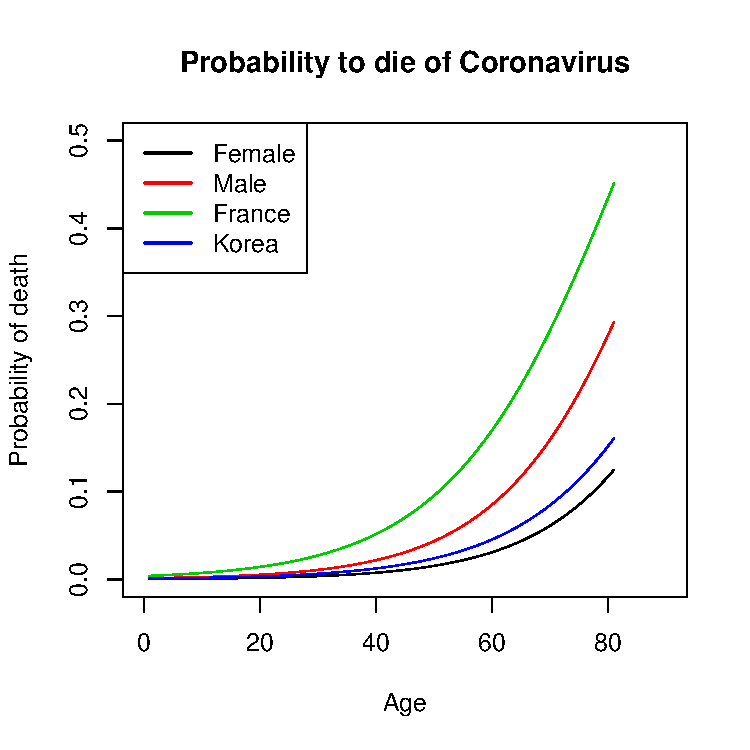
\includegraphics{Eksamensbesvarelse_files/figure-latex/unnamed-chunk-13-1.pdf}

\hypertarget{e}{%
\subsection{e)}\label{e}}

Without knowing how the data was collected, this is not a result we can
trust. We don't know how many were tested, and how sick people needed to
be to be tested. If France only tested the people that were
hospitalized, and the other countries tested more people with milder
symptons, then it makes sense for France to have a higher mortality
rate.

\hypertarget{f}{%
\subsection{f)}\label{f}}

\begin{enumerate}
\def\labelenumi{\roman{enumi})}
\tightlist
\item
  True ii) True iii) True? (sometimes it is more important that ppl that
  deafault loans are predicted to default, than that people who don't
  default are predicted to not default. men her sa stefanie at de er
  vektet likt) iv) False?? Not sure, might be useful. The error rate is
  not that high?
\end{enumerate}

\hypertarget{problem-3}{%
\section{Problem 3}\label{problem-3}}

\begin{Shaded}
\begin{Highlighting}[]
\NormalTok{id <-}\StringTok{ "1heRtzi8vBoBGMaM2-ivBQI5Ki3HgJTmO"}  \CommentTok{# google file ID}
\NormalTok{d.support <-}\StringTok{ }\KeywordTok{read.csv}\NormalTok{(}\KeywordTok{sprintf}\NormalTok{(}\StringTok{"https://docs.google.com/uc?id=%s&export=download"}\NormalTok{, }
\NormalTok{    id), }\DataTypeTok{header =}\NormalTok{ T)}
\CommentTok{# We only look at complete cases}
\NormalTok{d.support <-}\StringTok{ }\NormalTok{d.support[}\KeywordTok{complete.cases}\NormalTok{(d.support), ]}
\NormalTok{d.support <-}\StringTok{ }\NormalTok{d.support[d.support}\OperatorTok{$}\NormalTok{totcst }\OperatorTok{>}\StringTok{ }\DecValTok{0}\NormalTok{, ]}
\end{Highlighting}
\end{Shaded}

\hypertarget{a-2}{%
\subsection{a)}\label{a-2}}

\begin{Shaded}
\begin{Highlighting}[]
\KeywordTok{hist}\NormalTok{(d.support}\OperatorTok{$}\NormalTok{totcst, }\DataTypeTok{plot =} \OtherTok{TRUE}\NormalTok{, }\DataTypeTok{main =} \StringTok{"Total cost"}\NormalTok{)}
\end{Highlighting}
\end{Shaded}

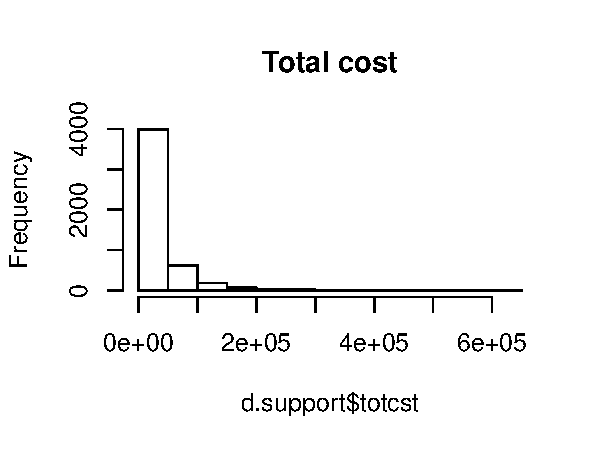
\includegraphics{Eksamensbesvarelse_files/figure-latex/unnamed-chunk-15-1.pdf}

\begin{Shaded}
\begin{Highlighting}[]
\KeywordTok{hist}\NormalTok{(d.support}\OperatorTok{$}\NormalTok{age, }\DataTypeTok{plot =} \OtherTok{TRUE}\NormalTok{, }\DataTypeTok{main =} \StringTok{"Age of patient"}\NormalTok{)}
\end{Highlighting}
\end{Shaded}

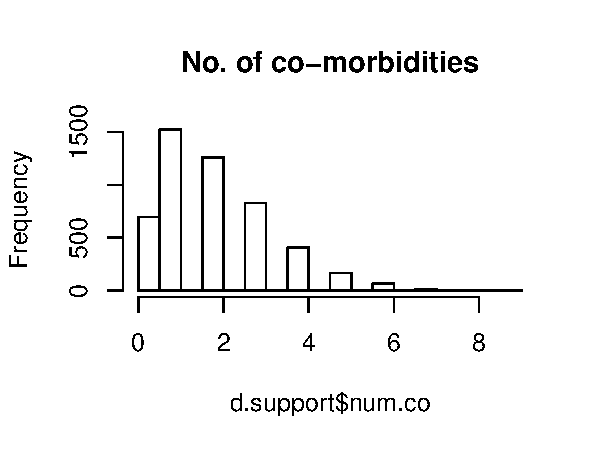
\includegraphics{Eksamensbesvarelse_files/figure-latex/unnamed-chunk-15-2.pdf}

\begin{Shaded}
\begin{Highlighting}[]
\KeywordTok{hist}\NormalTok{(d.support}\OperatorTok{$}\NormalTok{num.co, }\DataTypeTok{plot =} \OtherTok{TRUE}\NormalTok{, }\DataTypeTok{main =} \StringTok{"No. of co-morbidities"}\NormalTok{)}
\end{Highlighting}
\end{Shaded}

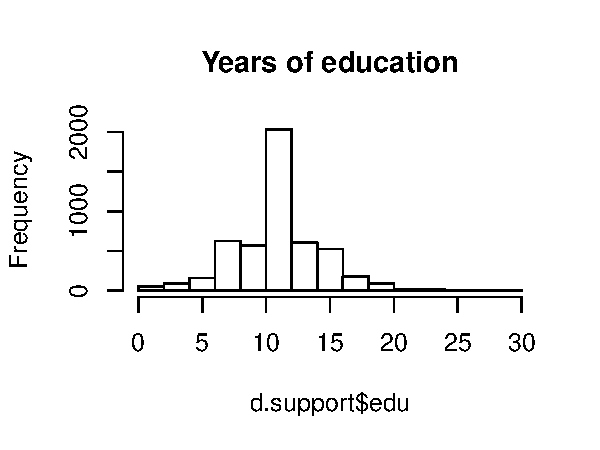
\includegraphics{Eksamensbesvarelse_files/figure-latex/unnamed-chunk-15-3.pdf}

\begin{Shaded}
\begin{Highlighting}[]
\KeywordTok{hist}\NormalTok{(d.support}\OperatorTok{$}\NormalTok{edu, }\DataTypeTok{plot =} \OtherTok{TRUE}\NormalTok{, }\DataTypeTok{main =} \StringTok{"Years of education"}\NormalTok{)}
\end{Highlighting}
\end{Shaded}

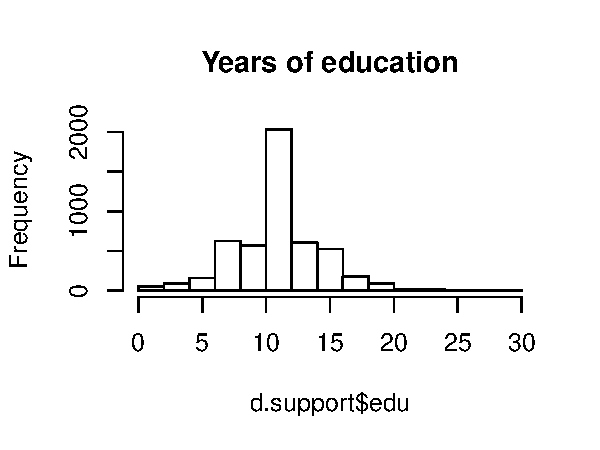
\includegraphics{Eksamensbesvarelse_files/figure-latex/unnamed-chunk-15-4.pdf}

\begin{Shaded}
\begin{Highlighting}[]
\KeywordTok{hist}\NormalTok{(d.support}\OperatorTok{$}\NormalTok{scoma, }\DataTypeTok{plot =} \OtherTok{TRUE}\NormalTok{, }\DataTypeTok{main =} \StringTok{"Measure fo Glasgow coma scale"}\NormalTok{)}
\end{Highlighting}
\end{Shaded}

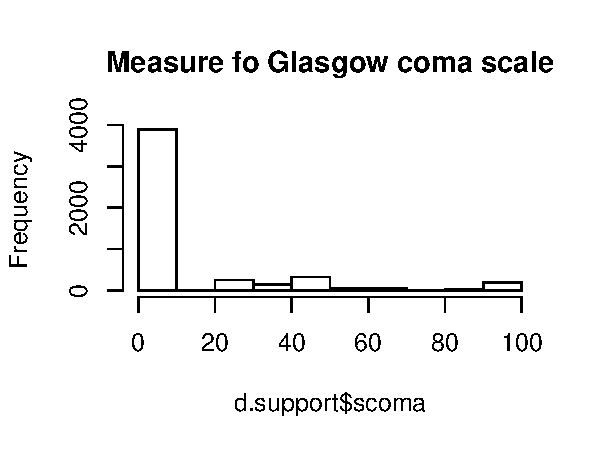
\includegraphics{Eksamensbesvarelse_files/figure-latex/unnamed-chunk-15-5.pdf}

\begin{Shaded}
\begin{Highlighting}[]
\KeywordTok{hist}\NormalTok{(d.support}\OperatorTok{$}\NormalTok{meanbp, }\DataTypeTok{plot =} \OtherTok{TRUE}\NormalTok{, }\DataTypeTok{main =} \StringTok{"Mean blood pressure"}\NormalTok{)}
\end{Highlighting}
\end{Shaded}

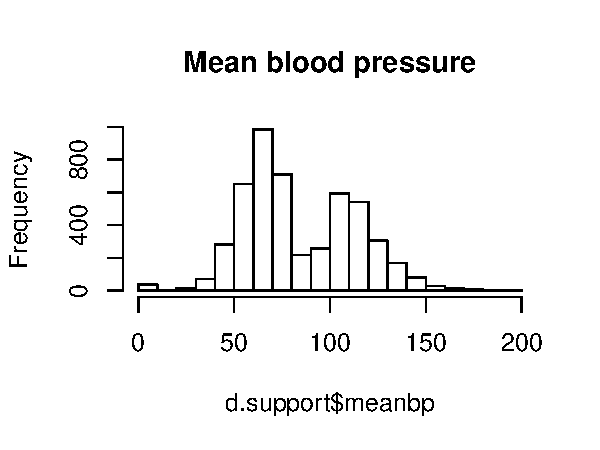
\includegraphics{Eksamensbesvarelse_files/figure-latex/unnamed-chunk-15-6.pdf}

\begin{Shaded}
\begin{Highlighting}[]
\KeywordTok{hist}\NormalTok{(d.support}\OperatorTok{$}\NormalTok{hrt, }\DataTypeTok{plot =} \OtherTok{TRUE}\NormalTok{, }\DataTypeTok{main =} \StringTok{"Heart rate"}\NormalTok{)}
\end{Highlighting}
\end{Shaded}

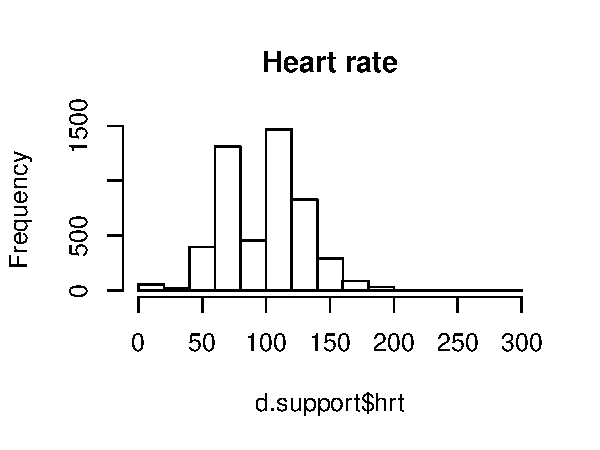
\includegraphics{Eksamensbesvarelse_files/figure-latex/unnamed-chunk-15-7.pdf}

\begin{Shaded}
\begin{Highlighting}[]
\KeywordTok{hist}\NormalTok{(d.support}\OperatorTok{$}\NormalTok{resp, }\DataTypeTok{plot =} \OtherTok{TRUE}\NormalTok{, }\DataTypeTok{main =} \StringTok{"Respatory frequency"}\NormalTok{)}
\end{Highlighting}
\end{Shaded}

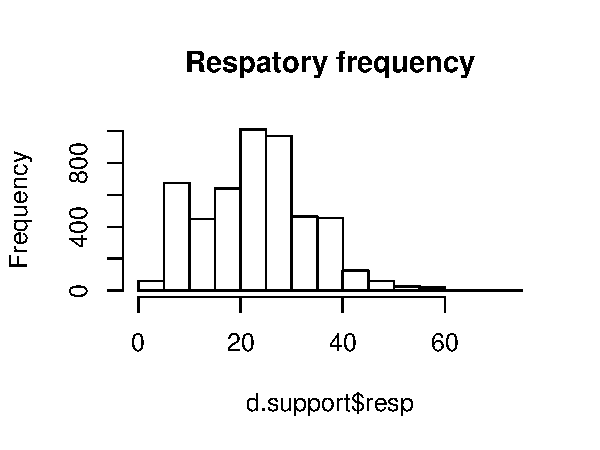
\includegraphics{Eksamensbesvarelse_files/figure-latex/unnamed-chunk-15-8.pdf}

\begin{Shaded}
\begin{Highlighting}[]
\KeywordTok{hist}\NormalTok{(d.support}\OperatorTok{$}\NormalTok{temp, }\DataTypeTok{plot =} \OtherTok{TRUE}\NormalTok{, }\DataTypeTok{main =} \StringTok{"Body temperature"}\NormalTok{)}
\end{Highlighting}
\end{Shaded}

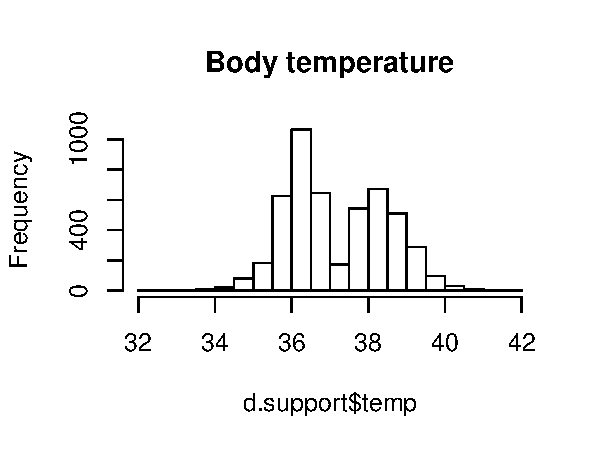
\includegraphics{Eksamensbesvarelse_files/figure-latex/unnamed-chunk-15-9.pdf}

\begin{Shaded}
\begin{Highlighting}[]
\KeywordTok{hist}\NormalTok{(d.support}\OperatorTok{$}\NormalTok{pafi, }\DataTypeTok{plot =} \OtherTok{TRUE}\NormalTok{, }\DataTypeTok{main =} \StringTok{"Pa02/Fi02 proportion"}\NormalTok{)}
\end{Highlighting}
\end{Shaded}

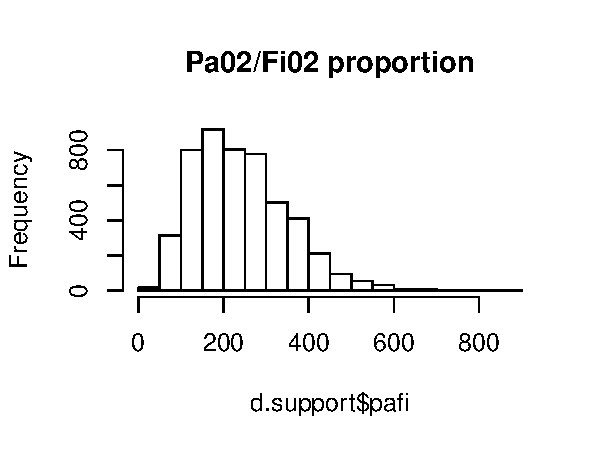
\includegraphics{Eksamensbesvarelse_files/figure-latex/unnamed-chunk-15-10.pdf}
I suggest a logarithmic transformation to the variable totcst, histogram
seen here:

\begin{Shaded}
\begin{Highlighting}[]
\KeywordTok{hist}\NormalTok{(}\KeywordTok{log}\NormalTok{(d.support}\OperatorTok{$}\NormalTok{totcst), }\DataTypeTok{plot =} \OtherTok{TRUE}\NormalTok{, }\DataTypeTok{main =} \StringTok{"Log of total cost"}\NormalTok{)}
\end{Highlighting}
\end{Shaded}

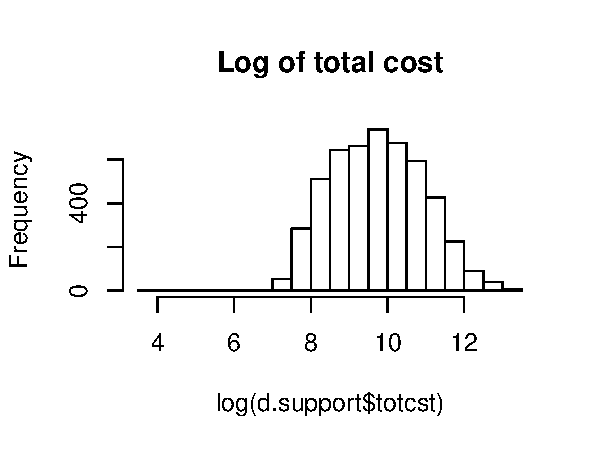
\includegraphics{Eksamensbesvarelse_files/figure-latex/unnamed-chunk-16-1.pdf}

\begin{Shaded}
\begin{Highlighting}[]
\CommentTok{# From now, we use the transformed version of totcst}
\NormalTok{d.support}\OperatorTok{$}\NormalTok{totcst =}\StringTok{ }\KeywordTok{log}\NormalTok{(d.support}\OperatorTok{$}\NormalTok{totcst)}
\end{Highlighting}
\end{Shaded}

\hypertarget{b-2}{%
\subsection{b)}\label{b-2}}

\begin{Shaded}
\begin{Highlighting}[]
\NormalTok{fit =}\StringTok{ }\KeywordTok{glm}\NormalTok{(totcst }\OperatorTok{~}\StringTok{ }\NormalTok{age }\OperatorTok{+}\StringTok{ }\NormalTok{temp }\OperatorTok{+}\StringTok{ }\NormalTok{edu }\OperatorTok{+}\StringTok{ }\NormalTok{resp }\OperatorTok{+}\StringTok{ }\NormalTok{num.co }\OperatorTok{+}\StringTok{ }\NormalTok{dzgroup, }\DataTypeTok{data =}\NormalTok{ d.support)}
\KeywordTok{summary}\NormalTok{(fit)}
\end{Highlighting}
\end{Shaded}

\begin{verbatim}
## 
## Call:
## glm(formula = totcst ~ age + temp + edu + resp + num.co + dzgroup, 
##     data = d.support)
## 
## Deviance Residuals: 
##     Min       1Q   Median       3Q      Max  
## -6.6554  -0.6524  -0.0437   0.6203   3.5226  
## 
## Coefficients:
##                       Estimate Std. Error t value Pr(>|t|)    
## (Intercept)          8.0823597  0.4014491  20.133  < 2e-16 ***
## age                 -0.0069950  0.0008742  -8.001 1.52e-15 ***
## temp                 0.0690123  0.0104548   6.601 4.51e-11 ***
## edu                  0.0249934  0.0039506   6.326 2.73e-10 ***
## resp                -0.0027792  0.0012791  -2.173   0.0298 *  
## num.co              -0.0430856  0.0107460  -4.009 6.18e-05 ***
## dzgroupCHF          -1.3992569  0.0437688 -31.969  < 2e-16 ***
## dzgroupCirrhosis    -0.9113548  0.0645311 -14.123  < 2e-16 ***
## dzgroupColon Cancer -1.4947386  0.0842719 -17.737  < 2e-16 ***
## dzgroupComa         -0.4501610  0.0562858  -7.998 1.57e-15 ***
## dzgroupCOPD         -1.2432540  0.0441240 -28.176  < 2e-16 ***
## dzgroupLung Cancer  -1.6924699  0.0540838 -31.293  < 2e-16 ***
## dzgroupMOSF w/Malig -0.2627110  0.0510358  -5.148 2.74e-07 ***
## ---
## Signif. codes:  0 '***' 0.001 '**' 0.01 '*' 0.05 '.' 0.1 ' ' 1
## 
## (Dispersion parameter for gaussian family taken to be 0.8718141)
## 
##     Null deviance: 6975.1  on 4959  degrees of freedom
## Residual deviance: 4312.9  on 4947  degrees of freedom
## AIC: 13410
## 
## Number of Fisher Scoring iterations: 2
\end{verbatim}

\begin{Shaded}
\begin{Highlighting}[]
\NormalTok{new_grid =}\StringTok{ }\KeywordTok{expand.grid}\NormalTok{(}\DataTypeTok{age =} \KeywordTok{c}\NormalTok{(}\DecValTok{10}\NormalTok{, }\DecValTok{20}\NormalTok{, }\DecValTok{30}\NormalTok{, }\DecValTok{40}\NormalTok{, }\DecValTok{50}\NormalTok{, }\DecValTok{60}\NormalTok{, }\DecValTok{70}\NormalTok{, }\DecValTok{80}\NormalTok{, }\DecValTok{90}\NormalTok{), }\DataTypeTok{temp =} \DecValTok{36}\NormalTok{, }\DataTypeTok{edu =} \DecValTok{10}\NormalTok{, }
    \DataTypeTok{resp =} \DecValTok{20}\NormalTok{, }\DataTypeTok{num.co =} \DecValTok{2}\NormalTok{, }\DataTypeTok{dzgroup =} \StringTok{"CHF"}\NormalTok{)}

\NormalTok{log_cost =}\StringTok{ }\KeywordTok{predict.glm}\NormalTok{(fit, }\DataTypeTok{newdata =}\NormalTok{ new_grid, }\DataTypeTok{type =} \StringTok{"response"}\NormalTok{)}
\NormalTok{cost =}\StringTok{ }\KeywordTok{exp}\NormalTok{(log_cost)}
\NormalTok{cost}
\end{Highlighting}
\end{Shaded}

\begin{verbatim}
##        1        2        3        4        5        6        7        8 
## 9954.460 9281.939 8654.854 8070.134 7524.917 7016.536 6542.500 6100.491 
##        9 
## 5688.343
\end{verbatim}

\begin{enumerate}
\def\labelenumi{\roman{enumi})}
\item
  When a patient's age increases by 10 years, the cost increase by
  factor 0.93244 (or equivalently, decrease by factor 1.07245).
\item
\end{enumerate}

\begin{Shaded}
\begin{Highlighting}[]
\KeywordTok{plot}\NormalTok{(fit)}
\end{Highlighting}
\end{Shaded}

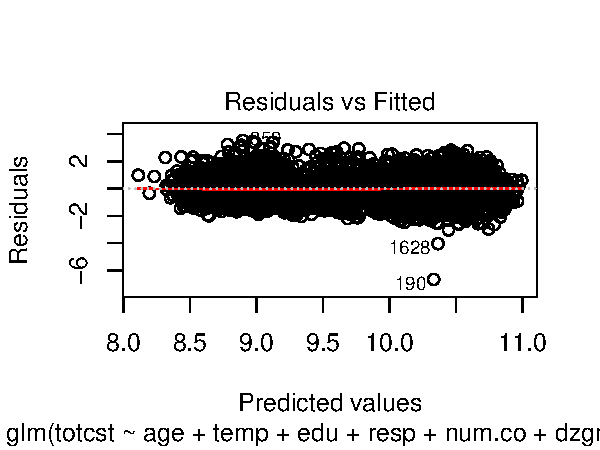
\includegraphics{Eksamensbesvarelse_files/figure-latex/unnamed-chunk-19-1.pdf}
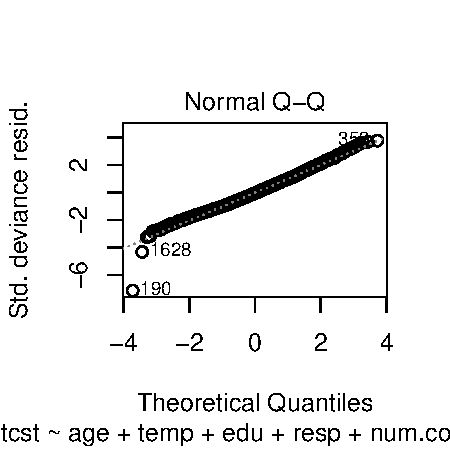
\includegraphics{Eksamensbesvarelse_files/figure-latex/unnamed-chunk-19-2.pdf}
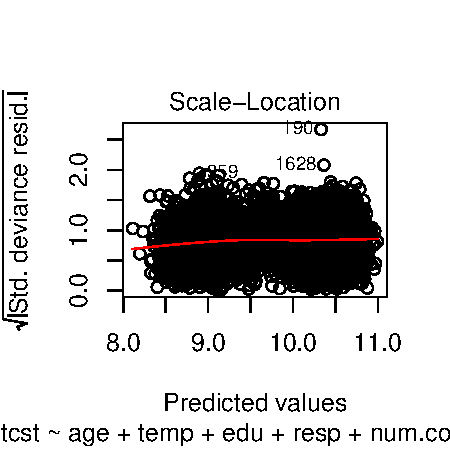
\includegraphics{Eksamensbesvarelse_files/figure-latex/unnamed-chunk-19-3.pdf}
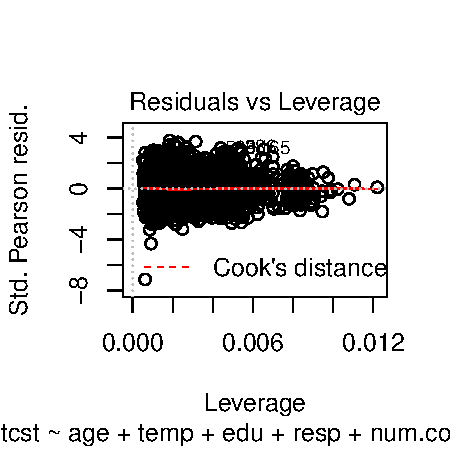
\includegraphics{Eksamensbesvarelse_files/figure-latex/unnamed-chunk-19-4.pdf}
We see from the Q-Q-diagram that the distibrution is normal, and not
skewed. We see from the residuals vs.~fitted-plot that there is no clear
pattern, indicating that the assumptions in the model are fulfilled.

\begin{enumerate}
\def\labelenumi{\roman{enumi})}
\setcounter{enumi}{2}
\item
\end{enumerate}

\hypertarget{c-1}{%
\subsection{c)}\label{c-1}}

\begin{Shaded}
\begin{Highlighting}[]
\KeywordTok{set.seed}\NormalTok{(}\DecValTok{12345}\NormalTok{)}
\NormalTok{train.ind =}\StringTok{ }\KeywordTok{sample}\NormalTok{(}\DecValTok{1}\OperatorTok{:}\KeywordTok{nrow}\NormalTok{(d.support), }\FloatTok{0.8} \OperatorTok{*}\StringTok{ }\KeywordTok{nrow}\NormalTok{(d.support))}
\NormalTok{d.support.train =}\StringTok{ }\NormalTok{d.support[train.ind, ]}
\NormalTok{d.support.test =}\StringTok{ }\NormalTok{d.support[}\OperatorTok{-}\NormalTok{train.ind, ]}
\end{Highlighting}
\end{Shaded}

\hypertarget{d-1}{%
\subsection{d)}\label{d-1}}

\hypertarget{e-1}{%
\subsection{e)}\label{e-1}}

\hypertarget{problem-4}{%
\section{Problem 4}\label{problem-4}}

\hypertarget{a-3}{%
\subsection{a)}\label{a-3}}

Basis functions: \$\$ b\_1(x) = X \text{, } b\_2(x) = X\^{}2 \text{, }
b\_3(x) = X\^{}3 \text{, } b\_4(x) = (X-1)\emph{+\^{}3 \text{, } b\_5(x)
= (X-2)}+\^{}3.

\[
Design matrix: Usikker på hvordan jeg skal gjøre det... Skal det være en nxp-matrise, skal det være subskript på x-ene? Skal jeg bruke bs()? tror jeg skal skrive for hånd.. 
\]

\textbackslash begin\{bmatrix\} 1 \& x\_1 \& x\_1\^{}2 \& x\_1\^{}3 \&
(x\_1-1)\emph{+\^{}3 \& (x\_1-2)}+\^{}3 \textbackslash{} 1 \& x\_2 \&
x\_2\^{}2 \& x\_2\^{}3 \& (x\_2-1)\emph{+\^{}3 \& (x\_2-2)}+\^{}3
\textbackslash{} \vdots \& \vdots \& \vdots \& \vdots \& \vdots \&
\vdots \textbackslash{} 1 \& x\_n \& x\_n\^{}2 \& x\_n\^{}3 \&
(x\_n-1)\emph{+\^{}3 \& (x\_n-2)}+\^{}3 \textbackslash{}
\textbackslash end\{bmatrix\}

\$\$

\hypertarget{b-3}{%
\subsection{b)}\label{b-3}}

\begin{enumerate}
\def\labelenumi{\roman{enumi})}
\tightlist
\item
  True ii) True iii) True iv) False
\end{enumerate}

\hypertarget{c-2}{%
\subsection{c)}\label{c-2}}

\begin{enumerate}
\def\labelenumi{\roman{enumi})}
\tightlist
\item
  False ii) False iii) False? (too small difference r) iv) False
\end{enumerate}

\hypertarget{problem-5}{%
\section{Problem 5}\label{problem-5}}

\hypertarget{a-4}{%
\subsection{a)}\label{a-4}}

\begin{enumerate}
\def\labelenumi{\roman{enumi})}
\tightlist
\item
  True, ii) True, iii) False, iv) Unsure (You can use reg, but is it a
  method for reg?)
\end{enumerate}

\hypertarget{b-4}{%
\subsection{b)}\label{b-4}}

\begin{enumerate}
\def\labelenumi{\roman{enumi})}
\tightlist
\item
  False ii) True iii) False iv) True?
\end{enumerate}

\hypertarget{c-single-choice}{%
\subsection{c) Single choice}\label{c-single-choice}}

True: iv)

\hypertarget{d-single-choice}{%
\subsection{d) Single choice}\label{d-single-choice}}

True: ii)

\hypertarget{e-single-choice}{%
\subsection{e) Single choice}\label{e-single-choice}}

True: iv)

\hypertarget{f-1}{%
\subsection{f)}\label{f-1}}

\begin{enumerate}
\def\labelenumi{\roman{enumi})}
\tightlist
\item
  True ii) False ? (can happen, but not always true. as sensitivity
  increases, specificity doesn't HAVE to go down) iii) False iv) True
\end{enumerate}

\hypertarget{g}{%
\subsection{g)}\label{g}}

\begin{enumerate}
\def\labelenumi{\roman{enumi})}
\tightlist
\item
  False ii) True iii) True iv) True
\end{enumerate}

\end{document}
